\documentclass[a4paper,10pt]{article}

\usepackage[activeacute]{babel}
\usepackage[utf8]{inputenc}
\usepackage{bookman}
\usepackage{color}
\usepackage{graphicx,wrapfig}
\usepackage{anysize}
\usepackage[pdftex=true,colorlinks=true,linkcolor=black,urlcolor=blue,bookmarksopen=true]{hyperref}
\usepackage{bookmark}
\usepackage{enumitem,pifont}
\usepackage{amssymb,amsmath,mathtools,cancel}
\usepackage[dvipsnames]{xcolor}

\begin{document}

\newcommand{\HRule}{\rule{\linewidth}{0.5mm}}

\begin{figure}[t]
\begin{center}
    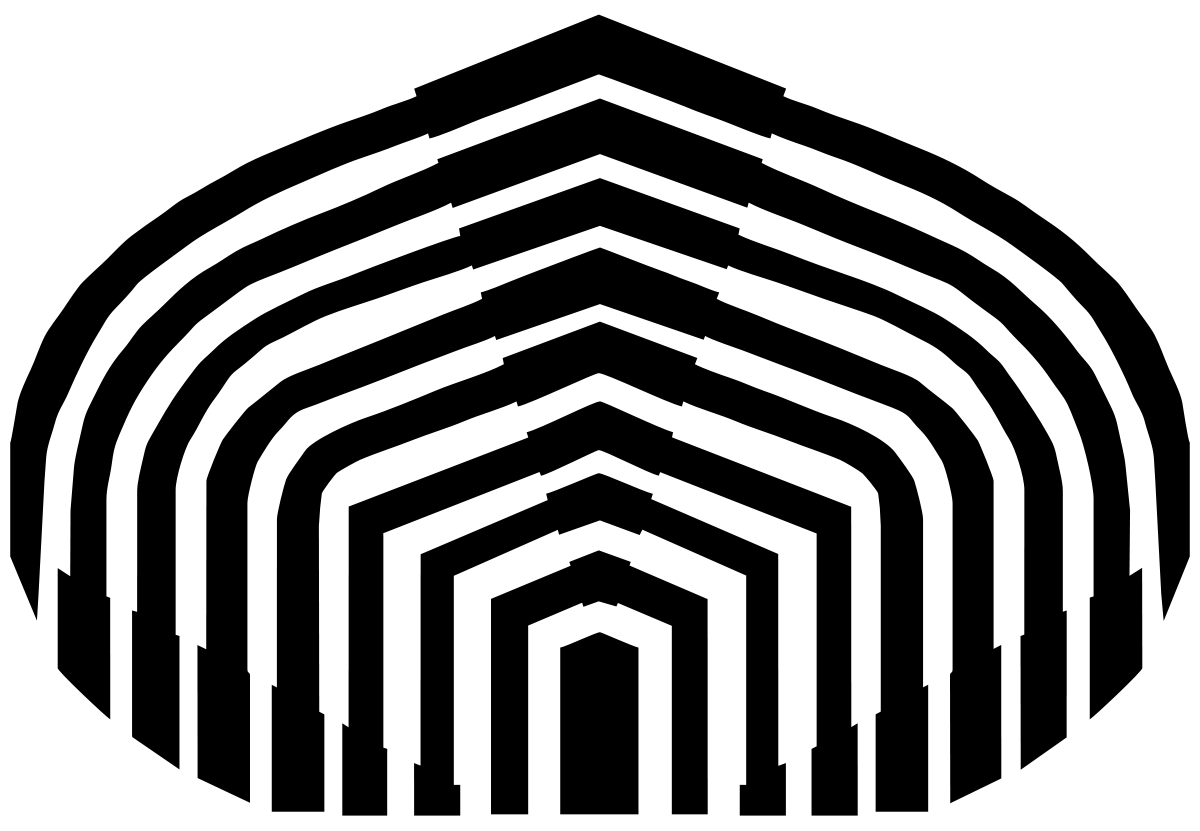
\includegraphics[scale=0.07]{USB.png}\\[0.6cm]
    \textsc
    {
        \LARGE Universidad Simón Bolívar \\[0.5cm]
    }
    \HRule \\[0.4cm]
    {\huge \bfseries Unidad II: Fen\'omenos el\'ectricos bajo distintos modelos} \\[0.4cm]
    
    Junior Zambrano\\[0.05cm]
    e-mail: 18-10929@usb.ve\\[0.2cm]
    \textsc{
    Julio de 2021
    }
\end{center}
\end{figure}

\renewcommand{\abstractname}{Prefacio}
\begin{abstract}
    El presente es un compendio te\'orico de la segunda unidad del curso
    \textbf{F\'isica 3 (FS-2211)} que trata de los fen\'omenos el\'ectricos bajo
    distintos modelos, que fue elaborado a partir de apuntes, notas y s\'intesis de
    las clases dictadas por el profesor \textbf{Sttiwuer D\'iaz} mientras dictaba
    dicho curso durante el trimestre \textbf{Abril-Julio 2021}.

    Entre los temas que se abordan est\'an, modelos de acci\'on a distancia, Ley de Coulomb,
    fuerza el\'ectrica, modelo de campo el\'ectrico, propiedades de los campos el\'ectricos,
    l\'ineas de campo el\'ectrico, campo el\'ectrico producido por una carga puntual y
    movimiento en un campo el\'ectrico uniforme.

    Cualquier error y/o sugerencia, por favor notificar al autor de este documento.
\end{abstract}

\renewcommand{\labelitemi}{\ding{226}}

% Clase 9

\section*{Clase 9: Modelo de acci\'on a distancia I}

\begin{itemize}

\subsection*{Modelos de acción a distancia}

\item La interacci\'on se propaga a velocidad infinita.

\item La interacción entre dos cuerpos depende de la distancia relativa entre ambos.

\item Si muevo aunque sea un poco uno de los cuerpos, ¿el otro ser\'a capaz de enterarse
de la modificaci\'on? S\'i lo hace y se entera inmediatamente en el momento de la perurbaci\'on,
por esta razón decimos que el cambio de la interacci\'on se transmite a velocidad infinita.

\textbf{Nota:} La velocidad realmente es finita y corresponde a la de la velocidad de la luz.

\item El fot\'on es el mediador de las interacciones el\'ectricas. Podr\'ia considerarse el
mensajero de la informaci\'on entre las dos cargas.

\item Este modelo de acci\'on est\'a en desuso actualmente porque no representa una
descripci\'on adecuada de la realidad.

\item La Ley de Gravitaci\'on Universal es un ejemplo de modelo de acci\'on a distancia.

\subsection*{Ley de Coulomb}

\item A partir de los experimentos de Charles Coulomb en 1975 se establece la interacci\'on
el\'ectrica que experimentan dos cuerpos cargados que se mantienen en reposo. Las conclusiones
fueron las siguientes:

\item La intensidad de la fuerza ele\'ectrica es inversamente proporcional a la distancia al
cuadrado que separa las cargas.

\begin{equation*}
    \boxed{\left\lvert\vec{F}_{ij}\right\lvert\varpropto
    \left\lvert\vec{r}_{ji}\right\lvert^{-2}=
    \frac{1}{\left\lvert\vec{r}_{ji}\right\lvert^2}}
\end{equation*}

\item La intensidad de la fuerza ele\'ectrica es directamente proporcional al valor de la
carga en valor absoluto.

\begin{equation*}
    \boxed{\left\lvert\vec{F}_{ij}\right\lvert\varpropto
    \left\lvert q_{i}q_{j}\right\lvert=\left\lvert q_{i}\right\lvert
    \left\lvert q_{j}\right\lvert}
\end{equation*}

\item La fuerza el\'ectrica es del tipo atractiva cuando las cargas tienen signos opuestos.

\item La fuerza el\'ectrica es del tipo repulsiva cuando las cargas tienen signos iguales.

\item Aunque el modelo de Coulomb es v\'alido s\'olo cuando las cargas el\'ectricas est\'an
en reposo, si la carga que est\'a ejerciendo la fuerza se encuentra inm\'ovil (en reposo)
y la carga sobre la cual se est\'a ejerciendo la fuerza se est\'a moviendo, entonces 
es posible usar este modelo de acci\'on.

\item El vector fuerza $\vec{F}_{ij}$ es colinial al vector de la distancia relativa entre
las cargas $\vec{r}_{ji}$, siendo paralelo cuando las cargas son distintas y antiparalelo
cuando son diferentes.

\begin{equation*}
    \boxed{\vec{F}_{ij}\varpropto
    \frac{q_{i}q_{j}}{\left\lvert\vec{r}_{ji}\right\lvert^2}\hat{r}_{ji}=
    \frac{q_{i}q_{j}}{\left\lvert\vec{r}_{ji}\right\lvert^3}\vec{r}_{ji}}
\end{equation*}

Donde $\hat{r}_{ji}=\dfrac{\vec{r}_{ji}}{\left\lvert\vec{r}_{ji}\right\lvert}$ es el vector
unitario dirigido desde la carga $q_i$ hasta la carga $q_j$.

\item Estas tres propiedades podemos resumirla en una sola expresi\'on:

\begin{equation*}
    \boxed{\vec{F}_{ij}=
    K_\varepsilon\frac{q_{i}q_{j}}{\left\lvert\vec{r}_{ji}\right\lvert^2}\hat{r}_{ji}=
    K_\varepsilon\frac{q_{i}q_{j}}{\left\lvert\vec{r}_{ji}\right\lvert^3}\vec{r}_{ji}}
\end{equation*}

Donde $\vec{r}_{ji}\stackrel{\mathrm{def}}{=}r_{j}-r_{i}$ es la
posici\'on relativa de la carga $q_j$ respecto a la carga $q_i$,
$r_{i}$ la posici\'on de la carga $q_i$ que ejerce la fuerza el\'ectrica y $r_{j}$
la posici\'on de la carga $q_j$ sobre la que act\'ua la fuerza.

\item La constante de propocionalidad $K_{e}$ depende del vac\'io (regi\'on del espacio en el
cual se ha extra\'ido toda mol\'ecula de aire).

\begin{equation*}
    \boxed{K_e=\frac{1}{4\pi\varepsilon_0}=9\times10^9\frac{Nm^2}{C^2}}
\end{equation*}

\item En caso que las cargas se encuentren en un medio distinto del vac\'io, la constante
$K$ viene dada por:

\begin{equation*}
    \boxed{K=\frac{1}{\kappa}=\frac{\varepsilon_0}{\varepsilon}}
\end{equation*}

Donde $\kappa=\frac{\varepsilon}{\varepsilon_0}$ es la constante diel\'ectrica y $\varepsilon$ la
constante de permitividad en se medio.

\item La fuerza el\'ectrica tiene unidades de newton, es decir, $N$.

\end{itemize}

% Clase 10

\section*{Clase 10: Modelo de acci\'on a distancia II}

\subsection*{Principio de superposici\'on}

\begin{itemize}

\item La fuerza el\'ectrica total ejercida sobre una carga se consigue sumando vectorialmente
las fuerzas el\'ectricas que ejercen sobre ella el conjunto de cargas restantes del sistema.

\begin{equation*}
    \boxed{\vec{F}_i=\vec{F}_{i1}+\vec{F}_{i2}+\cdots+\vec{F}_{i(1-N)}+\vec{F}_{iN}=
    \sum_{j=1\\j\neq i}^{N}\vec{F}_{ij}}
\end{equation*}

\item Esto implica que la aparici\'on de una tercera carga no afecta la interacci\'on de
dos cargas.

\item Una fuerza media la interacci\'on rec\'iproca entre el cuerpo que la esta ejerciendo y
sobre el cual est\'a actuando.

\item La suma de todas estas fuerzas no es una fuerza real; se trata de una pseudo fuerza
porque no cumple con la tercera ley de Newton.

\end{itemize}

% Clase 11

\section*{Clase 11: Fuerza el\'ectrica debido a distribuciones continuas}

\begin{itemize}

\item Se toma un diferencial de carga $dq$ de la distribuci\'on continua que represente a la
carga puntual que ejerce la fuerza el\'ectrica.

\item La posición relativa de la carga puntual $Q_0$ respecto a $dq$ se determina como es
usual, donde $\vec{r}_dq$ se obtiene parametrizando el espacio $\varepsilon$ que la contiene. 

\item La fuerza el\'ectrica que ejerce una distribuci\'on continua de carga sobre una
part\'icula puntual queda descrita por:

\begin{equation*}
    \boxed{\vec{F}_{Q_0}=K_\varepsilon Q_{0}\int_{\varepsilon}\frac{\vec{r}_{Q_0}-\vec{r}_{dq}}
    {\left\lvert\vec{r}_{Q_0}-\vec{r}_{dq}\right\lvert^3}\mathcal{D}_{Q}\mathrm{d}e}
\end{equation*}

\end{itemize}

% Clase 12

\section*{Clase 12: Modelo de campo el\'ectrico I}

\subsection*{Modelo de acci\'on de campo}

\begin{itemize}

\item Acci\'on de campo: la interacci\'on se establece en cada punto del espacio $\vec{r}$ y en un
instante de tiempo $t$.

\item Es un principio que est\'a basado en la localidad de las part\'iculas.

\item El campo interact\'ua con una part\'icula que est\'a colocada en una parte del espacio y la
interacci\'on viene dada por la perturbaci\'on que produce la part\'icula con la vencidad
en la que est\'a colocada.

\item El campo depende de los puntos en el espacio en el que fue colocado y si coloco una carga dentro del campo,
esta genera una fuerza electrost\'atica.

\item En concreto, el campo electrico en un punto $r$ del espacio en un instante de tiempo $t$ se va
a medir a partir de la interacción el\'ectrica que produce una part\'icula de prueba $q_0$ con el
entorno en el que est\'a ubicada, diviendo el valor de la fuerza el\'ectrica entre el valor
de la carga de prueba, independientemente del valor de la carga. Esto se logra tendiendo
la magnitud de la carga de prueba a cero.

\begin{equation*}
    \boxed{\vec{E}(\vec{r},t)=\lim_{q_0\to0}\frac{\vec{F}_{q_0}}{q_0}}
\end{equation*}

\item El campo el\'ectrico es una magnitud vectorial que tiene unidades de voltios por
metro, $\frac{V}{m}$, en el sistema MKS.

\end{itemize}

\subsection*{Propiedades generales del campo el\'ectrico}

\begin{itemize}

\item El valor del campo el\'ectrico es independiente de la carga de prueba.

\item Un campo es homog\'eneo cuando es independiento de los puntos del espacio,
pero puede mostrar dependencias respecto del tiempo.

\begin{equation*}
    \boxed{\vec{E}(\vec{r},t)=\vec{E}(t)\quad\forall r\in\mathbb{R}^3}
\end{equation*}

\item Un campo es constante cuando el campo el\'etrico puede cambiar en diferentes
puntos del espacio, pero al cambiar el tiempo es el mismo.

\begin{equation*}
    \boxed{\vec{E}(\vec{r},t)=\vec{E}(\vec{r})\quad\forall t\in\mathbb{R}}
\end{equation*}

\item Un campo es uniforme cuando es homog\'eneo y constante a la vez.
Es decir, que no depende ni de su posici\'on en el espacio ni del instante de tiempo.

\begin{equation*}
    \boxed{\vec{E}(\vec{r},t)=\vec{E}_0\quad\forall (\vec{r},t)\in\mathbb{R}^3}
\end{equation*}

\item Un campo es is\'otropo cuando la magnitud del campo no depende
de la direcci\'on del mismo en un origen com\'un.

\begin{equation*}
    \boxed{\left\lvert\vec{E}(\vec{r},t)\right\lvert=
    \left\lvert\vec{E}_0\right\lvert\quad\forall (\vec{r},t)\in\mathbb{R}^3
    \textrm{ tal que }R=\left\lvert\vec{r}\right\lvert}
\end{equation*}


\item El campo el\'ectrico cumple con el principio de superposici\'on, de modo
que:

\begin{equation*}
    \boxed{\vec{E}_i=\vec{E}_{i1}+\vec{E}_{i2}+\cdots+\vec{E}_{i(1-N)}+\vec{E}_{iN}=
    \sum_{j=1\\j\neq i}^{N}\vec{E}_{ij}}
\end{equation*}

\item El campo el\'ectrico que genera la superficie de un conductor con un exceso de carga
acumulada tiene la propiedad de ser perpendicular a dicha superficie, dirigi\'endose
afuera de esta si la carga es positiva y hacia dentro si la carga es negativa.

\item Una carga puntual que es colocada sobre una regi\'on de campo el\'etrico $\vec{E}$
experimenta una fuerza el\'ectrica dada por $\vec{F}=Q\vec{E}$, tal que la fuerza es
paralela al campo cuando el signo de la carga es positiva y antiparalela cuando el
signo es negativo.

\end{itemize}

% Clase 13

\section*{Clase 13: Modelo de campo el\'ectrico II}

\subsection*{Líneas de campo eléctrico}

\begin{itemize}

\item Las regiones de campo el\'ectrico pueden ser visualizadas como un conjunto de
l\'ineas con una orientaci\'on espec\'ifica.

\item El n\'umero de l\'ineas en el campo nos da una medida cualitativa de su intensidad.
Por ejemplo, la presencia de m\'as l\'ineas en una regi\'on de campo en comparaci\'on a otra
implica que la primera tiene mayor magnitud.

\item El vector tangente a la trayectoria de una l\'inea en una  posici\'on determinada,
es el vector del campo el\'ectrico medido en dicho punto.

\item Para hallar las l\'ineas de un campo el\'ectrico, se considera que el campo estacionario
es proporcional a un campo de velocidades.

\begin{equation*}
    \boxed{\vec{E}(\vec{r})=\varLambda\frac{\mathrm{d}\vec{r}}
    {\mathrm{d}\lambda}}
\end{equation*}

\end{itemize}

\subsection*{Campos electrostáticos}

\begin{itemize}

\item Son campos irrotacionales, que tienen rotor cero, y que no dependen
explícitamente del tiempo, es decir, tambi\'en son campos del tipo estacionario.

\begin{equation*}
    \boxed{\textrm{\ding{192} }\vec{E}(\vec{r},t)=\vec{E}(\vec{r})}
    \qquad\textrm{y}\qquad
    \boxed{\textrm{\ding{193} }\vec{\nabla}\times\vec{E}=\vec{0}}
\end{equation*}

\item Cuando un campo es irrotacional y estacionario es un campo conservativo.

\item Todo campo electrostático es conservativo y viceversa.

\end{itemize}

\subsection*{Campos el\'ectricos para cargas puntuales}

\begin{itemize}

\item Por la Ley de Coulomb es posible obtener el campo el\'ectrico que ejerce una
carga puntual $Q$ ubicada en $\vec{r}_Q$ sobre una carga de prueba $q_0$ en un punto $P$
de posici\'on $\vec{r}_P$:

\begin{equation*}
    \boxed{\vec{E}_P=
    \frac{\vec{F}_{Qq_0}}{q_0}=\frac{1}{\cancel{q_0}}K_\varepsilon\frac{Q\cancel{q_0}}
    {\left\lvert\vec{r}_{PQ}\right\lvert^3}\vec{r}_{PQ}=
    K_\varepsilon\frac{Q}{\left\lvert\vec{r}_{PQ}\right\lvert^3}\vec{r}_{PQ}}
\end{equation*}

\item El campo el\'ectrico generado por una carga puntual no es homog\'eneo.

\item Es estacionario siempre que la carga no dependa del tiempo.

\item No es uniforme por no ser homog\'eneo.

\item Es isotr\'opico respecto a la ubicaci\'on de la carga que lo genera.

\item Es electrost\'atico si es estacionario.

\end{itemize}

% Clase 15

\section*{Clase 15: Movimiento de carga en un campo}

\subsection*{Aceleraci\'on de una part\'icula cargada en presencia de un campo el\'ectrico}

\begin{itemize}

\item La aceleraci\'on lineal que experimenta un cuerpo con carga $Q$ y masa $m$ puede
representarse mediante la sumatoria de fuerzas externas el\'ectricas y mec\'anicas que act\'uan
sobre dicho cuerpo. En este caso la fuerza el\'ectrica es causa de estar en una regi\'on de
campo el\'ectrico.

\begin{equation*}
    \boxed{Q\vec{E}(\vec{r},t)+\vec{F}_{mec.}=m\vec{A}}
\end{equation*}

\end{itemize}

\subsection*{Movimiento de carga en un campo el\'ectrico uniforme}

\begin{itemize}

\item El campo el\'ectrico generado por dos placas conductoras cargadas uniformemente
en toda su longitud y que est\'an paralelas una a la otra es uniforme entre ellas mientras
m\'as alejado se est\'e de los bordes de las placas.

\item En ausencia de la fuerza gravitacional terrestre, la aceleraci\'on traslacional de un
cuerpo de carga $Q$ y masa $m$ por causa de la fuerza el\'ectrica producida por el campo
uniforme de magnitud $E_0$ ser\'ia:

\begin{equation*}
    \boxed{A=Q\frac{E_0}{m}}
\end{equation*}

\item Una partícula con carga neutra no var\'ia su trayectoria al atravesar dicha regi\'on
de campo el\'ectrico.

\item Por otro lado, una part\'icula con carga positiva se ver\'a atra\'ida por la placa de
signo opuesto y al ingresar a la regi\'on se desviar\'a en direcci\'on del campo,
describiendo la trayectoria de un lanzamiento de proyectil.

\item Para el caso de la part\'icula de carga negativa, esta se desviar\'a hacia la placa
positiva, en sentido contrario al campo, describiendo igualmente la misma trayectoria hasta
su destino.

\item Una part\'icula de mayor masa tendr\'a una trayectoria mucho m\'as prolongada que
una de masa m\'as pequeña. Esto es debido a que la aceleraci\'on de un cuerpo con mayor
masa ser\'a menor a la aceleraci\'on de uno de masa menor.

\item Por el mismo hecho, a la part\'icula de mayor masa le tomar\'ia m\'as tiempo llegar
a una de las placas comparado con una part\'icula de masa menor si ambas parten
de la misma altura con igual rapidez y en el mismo instante de tiempo.

\item Las ecuaciones de posición de las part\'iculas para cada instante de tiempo $t$ pueden
escribirse de modo que:

\begin{equation*}
    \begin{cases}
        x=x_{0}+v_{x_0}t+\dfrac{a_{x}}{2}t^2\Rightarrow x=x_{0}+v_{0}t\\
        y=y_{0}+v_{y_0}t+\dfrac{a_{y}}{2}t^2\Rightarrow y=y_{0}+\dfrac{Q}{2m}E_0t^2
    \end{cases}
\end{equation*}

Siempre que la part\'icula ingrese al campo con una velocidad inicial con solo componente
horizontal, se desprecien los efectos de borde de las placas conductoras y el campo el\'ectrico
tenga direcci\'on vertical.

\end{itemize}

\end{document}